\documentclass[border=0pt,10pt]{standalone}
\usepackage{tikz}
\usetikzlibrary{trees}
\renewcommand\rmdefault{\ttdefault}

\makeatletter
\newcount\dirtree@lvl
\newcount\dirtree@plvl
\newcount\dirtree@clvl
\def\dirtree@growth{%
  \ifnum\tikznumberofcurrentchild=1\relax
  \global\advance\dirtree@plvl by 1
  \expandafter\xdef\csname dirtree@p@\the\dirtree@plvl\endcsname{\the\dirtree@lvl}
  \fi
  \global\advance\dirtree@lvl by 1\relax
  \dirtree@clvl=\dirtree@lvl
  \advance\dirtree@clvl by -\csname dirtree@p@\the\dirtree@plvl\endcsname
  \pgf@xa=.2cm\relax
  \pgf@ya=-.5cm\relax
  \pgf@ya=\dirtree@clvl\pgf@ya
  \pgftransformshift{\pgfqpoint{\the\pgf@xa}{\the\pgf@ya}}%
  \ifnum\tikznumberofcurrentchild=\tikznumberofchildren
  \global\advance\dirtree@plvl by -1
  \fi
}

\tikzset{
  dirtree/.style={
    growth function=\dirtree@growth,
    every node/.style={anchor=north, font=\bfseries},
    every child node/.style={anchor=west},
    edge from parent path={(\tikzparentnode\tikzparentanchor) |- (\tikzchildnode\tikzchildanchor)}
  }
}
\makeatother

\begin{document}
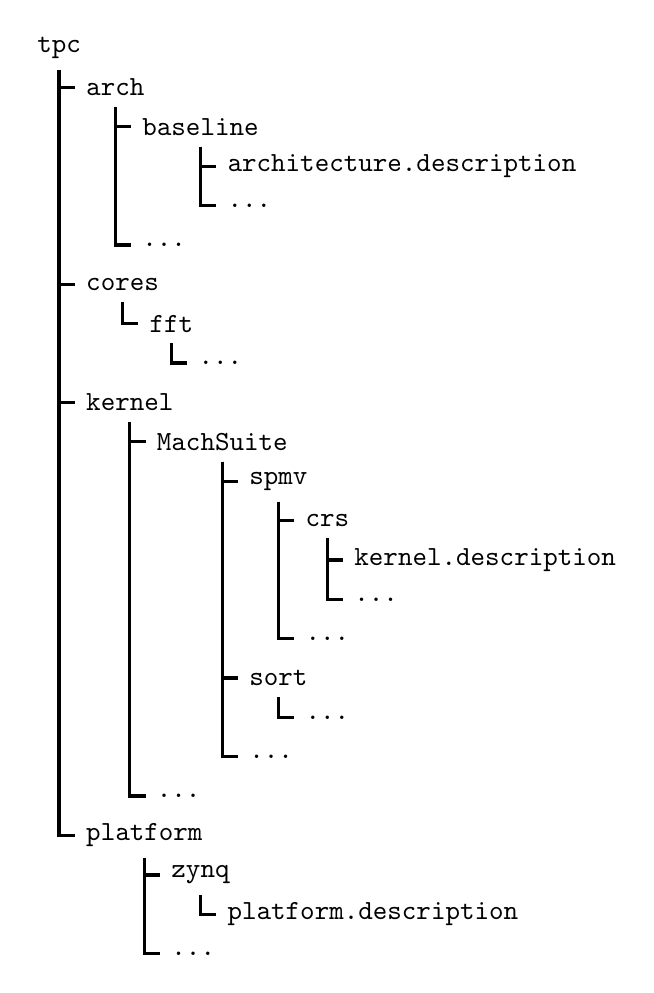
\begin{tikzpicture}[dirtree, line width=1.2pt]
\node {tpc} 
    child { node {arch}
            child { node {baseline}
	      child { node {architecture.description} }
	      child { node {\ldots} }
	    }
            child { node {\ldots} }
    }
    child { node {cores}
      child { node {fft} child { node {\ldots} }} }
    child { node {kernel}
%         child { node {add}
% 	  child { node {kernel.description} }
% 	  child { node {\ldots} }
% 	}
%         child { node {reader}
% 	  child { node {kernel.description} }
% 	  child { node {\ldots} }
% 	}
        child { node {MachSuite} 
	  child { node { spmv }
	    child { node {crs}
	      child { node {kernel.description} }
	      child { node {\ldots} }
            }
	    child { node {\ldots} }
	  }
	  child { node { sort } 
	    child { node {\ldots} }
	  }
	  child { node {\ldots} }
        }
	child { node {\ldots} }
    }
    child { node {platform}
        child { node {zynq}
	  child { node {platform.description} }
	}
        child { node {\ldots} }
    };
\end{tikzpicture}
\end{document}
